% Sequence layout visualization for PSE prefix injection on OpenVLA-7B.
% Compares (a) OpenVLA canonical, (b) PSSA variant_A (after_image),
% (c) PSSA variant_B (before_action). The eight position slots consumed
% by PSE are highlighted; this shifts downstream RoPE offsets by 8.
\documentclass[tikz,border=10pt]{standalone}
\usepackage{tikz}
\usepackage{xcolor}
\usetikzlibrary{positioning,backgrounds,fit,calc}

\definecolor{cBOS}{RGB}{100,100,100}
\definecolor{cIMG}{RGB}{56,103,214}
\definecolor{cPSE}{RGB}{210,90,40}
\definecolor{cTXT}{RGB}{36,128,68}
\definecolor{cEMPTY}{RGB}{200,200,80}
\definecolor{cACT}{RGB}{120,60,160}

\begin{document}
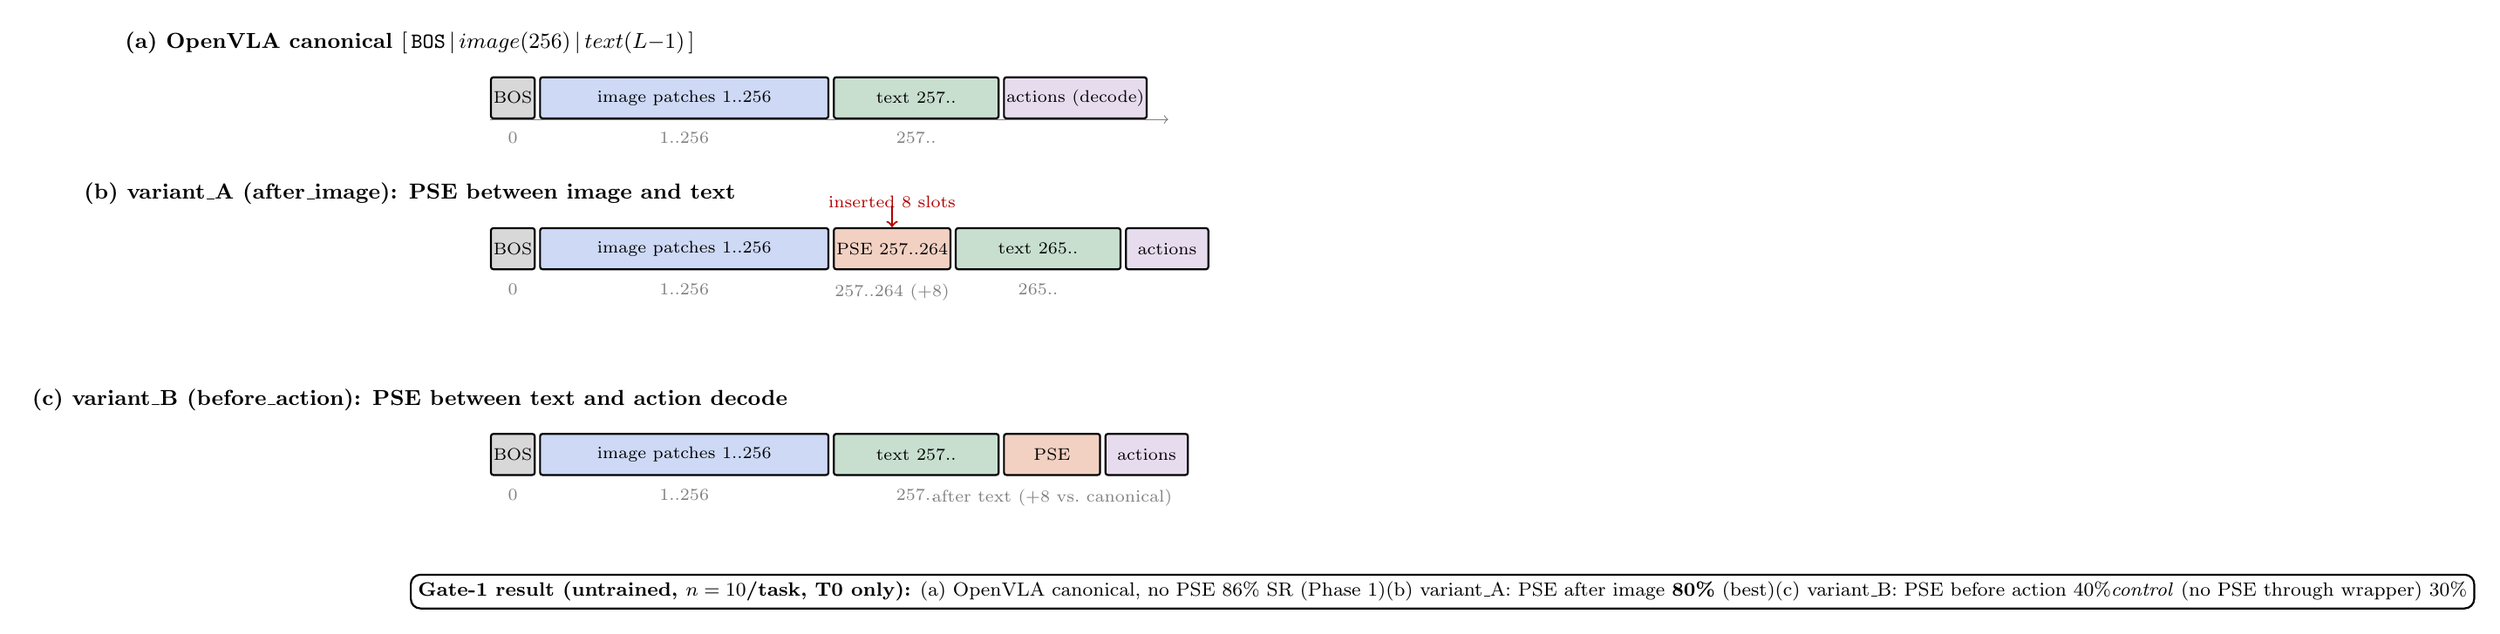
\begin{tikzpicture}[
    every node/.style={font=\scriptsize},
    tok/.style={draw,thick,rounded corners=1pt,minimum height=6mm,
                minimum width=5mm,inner sep=1pt,align=center},
    grp/.style={draw=none,inner sep=0pt},
]

% ====== Row 1: OpenVLA canonical (no PSE) ======
\node[font=\small\bfseries] (lab1) at (-0.5,3.0)
    {(a) OpenVLA canonical $[\,\texttt{BOS}\,|\,\text{image}(256)\,|\,\text{text}(L{-}1)\,]$};

\node[tok,fill=cBOS!25] (a_bos) at (1.0,2.2) {BOS};
\node[tok,fill=cIMG!25,minimum width=42mm,right=0.5mm of a_bos] (a_img) {image patches 1..256};
\node[tok,fill=cTXT!25,minimum width=24mm,right=0.5mm of a_img] (a_txt) {text 257..};
\node[tok,fill=cACT!18,minimum width=12mm,right=0.5mm of a_txt] (a_act) {actions (decode)};

% Position-index ruler
\draw[->,gray] (a_bos.south west) -- ($(a_act.south east)+(0.3,0)$);
\node[font=\scriptsize,gray,below=2pt of a_bos] {0};
\node[font=\scriptsize,gray,below=2pt of a_img] {1..256};
\node[font=\scriptsize,gray,below=2pt of a_txt] {257..};

% ====== Row 2: PSSA variant_A (after_image) ======
\node[font=\small\bfseries] (lab2) at (-0.5,0.8)
    {(b) variant\_A (after\_image): PSE between image and text};

\node[tok,fill=cBOS!25] (b_bos) at (1.0,0.0) {BOS};
\node[tok,fill=cIMG!25,minimum width=42mm,right=0.5mm of b_bos] (b_img) {image patches 1..256};
\node[tok,fill=cPSE!28,minimum width=14mm,right=0.5mm of b_img]  (b_pse) {PSE 257..264};
\node[tok,fill=cTXT!25,minimum width=24mm,right=0.5mm of b_pse] (b_txt) {text 265..};
\node[tok,fill=cACT!18,minimum width=12mm,right=0.5mm of b_txt] (b_act) {actions};

\node[font=\scriptsize,gray,below=2pt of b_bos] {0};
\node[font=\scriptsize,gray,below=2pt of b_img] {1..256};
\node[font=\scriptsize,gray,below=2pt of b_pse] {257..264 (+8)};
\node[font=\scriptsize,gray,below=2pt of b_txt] {265..};

% Highlight the PSE positions
\draw[->,red!70!black,thick] ($(b_pse.north)+(0,3mm)$) -- (b_pse.north)
    node[midway,above,red!70!black,font=\scriptsize] {inserted 8 slots};

% ====== Row 3: PSSA variant_B (before_action) ======
\node[font=\small\bfseries] (lab3) at (-0.5,-2.2)
    {(c) variant\_B (before\_action): PSE between text and action decode};

\node[tok,fill=cBOS!25] (c_bos) at (1.0,-3.0) {BOS};
\node[tok,fill=cIMG!25,minimum width=42mm,right=0.5mm of c_bos] (c_img) {image patches 1..256};
\node[tok,fill=cTXT!25,minimum width=24mm,right=0.5mm of c_img] (c_txt) {text 257..};
\node[tok,fill=cPSE!28,minimum width=14mm,right=0.5mm of c_txt] (c_pse) {PSE};
\node[tok,fill=cACT!18,minimum width=12mm,right=0.5mm of c_pse] (c_act) {actions};

\node[font=\scriptsize,gray,below=2pt of c_bos] {0};
\node[font=\scriptsize,gray,below=2pt of c_img] {1..256};
\node[font=\scriptsize,gray,below=2pt of c_txt] {257..};
\node[font=\scriptsize,gray,below=2pt of c_pse] {after text (+8 vs.\ canonical)};

% Result annotation
\node[draw,thick,rounded corners,fill=white,inner sep=3pt,
      anchor=west,font=\footnotesize,minimum width=70mm]
    at (-0.5,-5.0) {%
    \textbf{Gate-1 result (untrained, $n=10$/task, T0 only):}
    \\[1pt]
    (a) OpenVLA canonical, no PSE \dotfill 86\% SR (Phase~1) \\
    (b) variant\_A: PSE after image \dotfill \textbf{80\%} (best) \\
    (c) variant\_B: PSE before action \dotfill 40\% \\
    \emph{control} (no PSE through wrapper) \dotfill 30\%
};

\end{tikzpicture}
\end{document}
